\documentclass[a4paper,14pt]{extarticle}

\usepackage{geometry}
\usepackage{amsmath,bm}
\usepackage{amssymb}
\usepackage{amsthm}
\usepackage{esint}
\usepackage{float}
\usepackage{graphicx}
\usepackage[dvipsnames]{xcolor}
\usepackage[utf8]{inputenc}
\usepackage[T2A]{fontenc}
%\usepackage[lutf8x]{luainputenc}

%\usepackage{fontspec}
%\setmainfont{CMU Serif}
%\setsansfont{CMU Sans Serif}
%\setmonofont{CMU Typewriter Text}

\usepackage[greek.polutoniko,english,russian]{babel}
% локализация и переносы
\usepackage{latexsym}
\usepackage{hhline}
\usepackage{multirow}
\usepackage{vmargin,indentfirst} 
\setmarginsrb{20mm}{15mm}{15mm}{15mm}{0mm}{0mm}{0mm}{10mm}
\usepackage[multiple]{footmisc}
\usepackage{hyperref}
\usepackage{multirow}
\usepackage{pdflscape}
%\numberwithin{equation}{section}
\usepackage[labelsep=period]{caption}


% команда для переноса строки внутри ячейки таблицы
\newcommand{\specialcell}[2][l]{%
  \begin{tabular}[#1]{@{}l@{}}#2\end{tabular}}

  \usepackage{physics}

\usepackage{tikz}
\usetikzlibrary{calc}
\usetikzlibrary{arrows.meta}

%\usepackage[margin=0.3in,bmargin=0.5in]{geometry}

%\usepackage{CJKutf8}%Chinese characters


\pagestyle{plain}

\theoremstyle{plain}
\newtheorem{theorem}{Theorem}[section]
\newtheorem{lemma}[theorem]{Lemma}
\newtheorem*{proposition}{Proposition}
\newtheorem{corollary}[theorem]{Corollary}
\newtheorem{problem}[theorem]{Problem}
\newtheorem{exercise}{Exercise}[section]

\theoremstyle{remark}
\newtheorem*{example}{Example}
\newtheorem*{examples}{Examples}
\newtheorem*{remark}{Remark}
\newtheorem*{hint}{Hint}

\theoremstyle{definition}
\newtheorem*{definition}{Definition}

\renewcommand{\emptyset}{\varnothing}
\newcommand\ph{\varphi}
\newcommand\eps{\varepsilon}

\newcommand\mbZ{\mathbb Z}
\newcommand\mbC{\mathbb C}
\newcommand\mbR{\mathbb R}
\newcommand\mbN{\mathbb N}
\newcommand\mbQ{\mathbb Q}
\newcommand\mbE{\mathbb E}

\newcommand\mcB{\mathcal B}
\newcommand\mcC{\mathcal C}
\newcommand\mcF{\mathcal F}
\newcommand\mcG{\mathcal G}
\newcommand\mcJ{\mathcal J}


\newcommand\la{\langle}
\newcommand\ra{\rangle}
\newcommand\ol{\overline}
\newcommand\ora{\overrightarrow}
\newcommand\rsa{\rightsquigarrow}

\DeclareMathOperator{\M}{M}
\DeclareMathOperator{\Span}{Span}
\DeclareMathOperator{\LL}{\cal L}
\DeclareMathOperator{\id}{id}
\DeclareMathOperator{\Ker}{Ker}
\DeclareMathOperator{\Img}{Im}
\DeclareMathOperator{\rk}{rank}
%\DeclareMathOperator{\Tr}{Tr}
\DeclareMathOperator{\cof}{cof}

\newcommand\dfn[1]{{\bf #1}}
\renewcommand{\thesubsubsection}{}

\newcounter{saveenumi}
\newcommand{\seti}{\setcounter{saveenumi}{\value{enumi}}}
\newcommand{\conti}{\setcounter{enumi}{\value{saveenumi}}}

\newcommand{\vct}[1]{\overrightarrow{#1}}
\newcommand{\bvct}[1]{\boldsymbol{#1}}
\newcommand{\codir}{\upuparrows}
\newcommand{\ncodir}{\uparrow \downarrow }

%% title background

\DeclareMathOperator{\sign}{sign}
\DeclareMathOperator{\const}{const}
\newcommand{\dprodd}[2]{\vct{#1}\cdot\vct{#2}}
\newcommand{\dprod}[2]{\bvct{#1}\cdot\bvct{#2}}

\newcommand{\cprod}[2]{\bvct{#1}\times\bvct{#2}}

\newcommand{\mprod}[3]{(\bvct{#1},\bvct{#2},\bvct{#3})}

\newcommand{\vecsys}{{$\bvct{a}_1$ , . . . , $\bvct{a}_n$ {}}}

\newcommand{\Problem}[1]{\vspace{\baselineskip}\textbf{Problem {#1}}\par}
\newcommand{\Solution}{\vspace{\baselineskip}\textbf{Solution}\par}

\newcommand*\coord[1]{%
  \begin{pmatrix}
    #1
  \end{pmatrix}%
}

\renewcommand{\d}[1]{\ensuremath{\operatorname{d}\!{#1}}}

\usepackage{tkz-euclide}
%\usetkzobj{all}

\usepackage{subcaption}

\usepackage{enumitem}

\usepackage{datetime}
\newdateformat{yeardate}{\THEYEAR}

\usepackage[toc,page]{appendix}

\def\contentsname{Содержание}

\usepackage{listings}

\lstset{% Собственно настройки вида листинга
inputencoding=utf8, extendedchars=\true, keepspaces = true, % поддержка кириллицы и пробелов в комментариях
language=C++,            % выбор языка для подсветки (здесь это Pascal)
basicstyle=\small\sffamily, % размер и начертание шрифта для подсветки кода
numbers=left,               % где поставить нумерацию строк (слева\справа)
numberstyle=\tiny,          % размер шрифта для номеров строк
stepnumber=1,               % размер шага между двумя номерами строк
numbersep=5pt,              % как далеко отстоят номера строк от подсвечиваемого кода
backgroundcolor=\color{white}, % цвет фона подсветки - используем \usepackage{color}
showspaces=false,           % показывать или нет пробелы специальными отступами
showstringspaces=false,     % показывать или нет пробелы в строках
showtabs=false,             % показывать или нет табуляцию в строках
frame=single,               % рисовать рамку вокруг кода
tabsize=2,                  % размер табуляции по умолчанию равен 2 пробелам
captionpos=t,               % позиция заголовка вверху [t] или внизу [b] 
breaklines=true,            % автоматически переносить строки (да\нет)
breakatwhitespace=false,    % переносить строки только если есть пробел
escapeinside={\%*}{*)}      % если нужно добавить комментарии в коде
}
\begin{document}



% Оформление титульного листа
\begin{titlepage}
\begin{center}
\textsc{Санкт-Петербургский государственный университет\\
Математико-механический факультет\\
Кафедра физической механики\\}

\vfill

\textsc{Методы измерений и электромеханические системы\\[3mm]}
Отчёт по лабораторной работе №4\\[6mm]


\textbf{\large<<Проверка принципа эквивалентности масс>>}

\vfill
\end{center}

\hfill
\begin{minipage}{.5\textwidth}
Выполнил студент:\\[2mm] 
Кручинина Екатерина Васильевна\\
группа: 24.Б51-мм\\[5mm]

Проверил:\\[2mm] 
к.ф.-м.н., доцент\\
Кац Виктор Михайлович
\end{minipage}%
\vfill
\begin{center}
 Санкт-Петербург, \yeardate\today\ г.
\end{center}
\end{titlepage}
% Содержание
\tableofcontents
\newpage
\section{Введение}
\subsection{Цель работы}
Целью данной лабораторной работы является проверка принципа эквивалентности масс, измерение ускорения свободного падения тел и
знакомство с методом измерения интервалов времени между импульсами
частотомером – хронометром Ч3-32, а также определение погрешности косвенных измерений.

\subsubsection{Решаемые задачи}
В ходе выполнения работы решаются следующие задачи:
\begin{enumerate}
    \item Ознакомление с методом измерения интервалов времени между импульсами с помощью частотомера-хронометра Ч3-32.
    \item Измерение времени свободного падения тел из различных материалов (алюминий, латунь, сталь, дерево, плексиглас, свинец) на фиксированном участке пути.
    \item Вычисление ускорение свободного падения для каждого тела, на основе полученных данных.
    \item Проведение статистической обработки результатов измерений и оценивание погрешности прямых и косвенных измерений.
    \item Анализ полученных значений и формулировка вывода о справедливости принципа эквивалентности масс в условиях эксперимента.
\end{enumerate}

\newpage

\section{Основная часть}

\subsection{Теоретическая часть}

Как было установлено Галилеем, ускорение свободного падения одинаково для всех тел независимо от их массы и состава. Из этого результата следует равенство инертной и гравитационной масс.

Массу тела можно определить путем измерения испытываемого телом ускорения $\vec{a}$ под действием известной силы $\vec{F}$:
\begin{equation}
M_{\text{ин}} = \frac{|\vec{F}|}{|\vec{a}|}.
\end{equation}
Определяемая таким путем масса известна под названием инертной массы. Массу тела можно также определить, измеряя силу тяготения к другому телу, например, к Земле:
\begin{equation}
F = \gamma \frac{M_{\text{гр}} M_{\text{З}}}{r^2}, \quad M_{\text{гр}} = \frac{F r^2}{\gamma M_{\text{З}}},
\end{equation}
где $\gamma$ — гравитационная постоянная, $M_{\text{З}}$ — масса Земли, $r$ — расстояние между центром Земли и телом. 
Определяемая таким образом масса $M_{\text{гр}}$ называется гравитационной массой.

Докажем, что $M_{\text{гр}} = M_{\text{ин}}$ для любого тела. Для этого рассмотрим тело 1 с массой $M_{\text{ин}}^{(1)}$ и $M_{\text{гр}}^{(1)}$, падающее вблизи поверхности Земли. Тогда имеем:
\begin{equation}
M_{\text{ин}}^{(1)} a_1 = \gamma \frac{M_{\text{гр}}^{(1)} M_{\text{З}}}{R_{\text{З}}^2}, \tag{1}
\end{equation}
для тела 2 с $M_{\text{ин}}^{(2)}$ и $M_{\text{гр}}^{(2)}$:
\begin{equation}
M_{\text{ин}}^{(2)} a_2 = \gamma \frac{M_{\text{гр}}^{(2)} M_{\text{З}}}{R_{\text{З}}^2}. \tag{2}
\end{equation}
Поделив (1) на (2), получим:
\begin{equation}
\frac{M_{\text{ин}}^{(1)}} {M_{\text{ин}}^{(2)}}
\cdot \frac {a_1} {a_2} = \frac{M_{\text{гр}}^{(1)}}{M_{\text{гр}}^{(2)}}.
\end{equation}
Поскольку из закона Галилея следует, что $a_1 = a_2 = g$, то:
\begin{equation}
\frac{M_{\text{ин}}^{(1)}}{M_{\text{ин}}^{(2)}} = \frac{M_{\text{гр}}^{(1)}}{M_{\text{гр}}^{(2)}} ; \frac{M_{\text{ин}}^{(1)}}{M_{\text{гр}}^{(1)}} = \frac{M_{\text{ин}}^{(2)}}{M_{\text{гр}}^{(2)}} = \text{const}. \tag{3}
\end{equation}
Так как это отношение постоянно для всех тел, можно всегда привести его к единице, подобрав подходящее значение к гравитационной постоянной $\gamma$. Современные эксперименты с точностью до $10^{-12}$ подтвердили равенство инертной и гравитационной масс.

В 1915 году А. Эйнштейн сформулировал основные положения общей теории относительности для описания гравитационных явлений. Фундаментом этой теории является принцип эквивалентности, в основе которого лежит закон $M_{\text{гр}} = M_{\text{ин}}$.

В данной работе этот принцип проверяется косвенно: если он справедлив, то время пролета фиксированного расстояния $h$ для тел разной массы будет одинаковым. Уравнение движения шарика при свободном падении имеет вид:
\begin{equation}
h = v_0 t + \frac{gt^2}{2},
\end{equation}
откуда ускорение свободного падения можно выразить как:
\begin{equation}
g = \frac{2(h - v_0 t)}{t^2}. \tag{1}
\end{equation}
Здесь $v_0$ — начальная скорость шарика в момент пересечения верхнего светового луча.

\subsection{Эксперимент}
\subsubsection{Описание экспериментальной установки:}
Схема эксперементальной установки приведена на рис. 1. Луч от квантового генератора ЛГ направляется на призму полного внутреннего отражения П1, от нее на призму П2, а затем на фотодиод ФД. При отодвигании заслонки З шарик, находящийся в трубке Т, падает в лузу Л и пересекает два световых луча, расстояние между которыми равно h . Когда шарик пересекает верхний луч, фотодиод ФД вырабатывает импульс, который усилившись в усилителе, подается на вход частотомера Ч3-32 и запускает его. При пересечении шариком нижнего луча импульс от фотодиода останавливает счет частотомера. Интервал времени между двумя импульсами, регистрируемый
частотомером, равен времени пролета t шарика от верхнего луча до нижнего. Усилитель питается от источника УПУ-1У4.


\begin{figure}[H]
    \centering
    \begin{tabular}{c}
        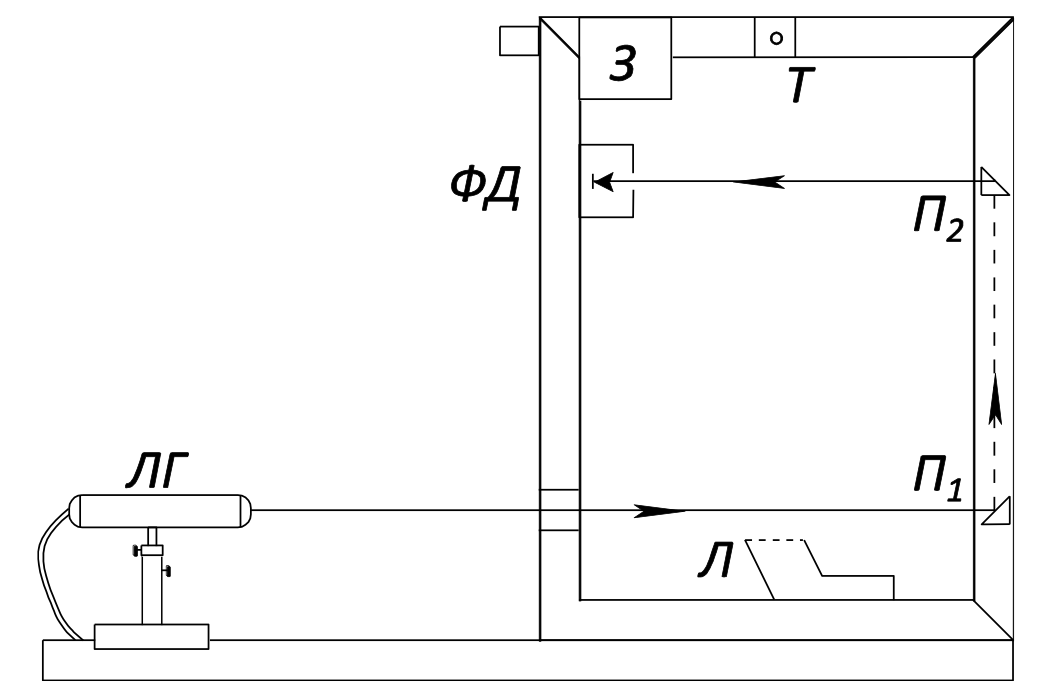
\includegraphics[width=0.6\textwidth]{эксп.установка.png} \\
    \end{tabular}
    \caption{Схема экспериментальной установки}
    \label{fig:setup}
\end{figure}

В работе используются шарики одинакового диаметра $d = 10$ мм из различных материалов: алюминий, латунь, сталь, дерево, плексиглас, свинец. Для каждого шарика проведена серия из 30 измерений времени пролета.


\textbf{Параметры установки:}

Расстояние между лучами: $h = (0,272 \pm 0,001)$ м

Начальная скорость: $v_0 = (1,052 \pm 0,005)$ м/с

Диаметр шариков: $d = 10$ мм


\subsection{Обработка результатов измерений}

\subsubsection{Таблицы}
В ходе эксперимента были получены данные, представленные в таблицах ниже.

\begin{table}[H]
\centering
\caption{Масса шариков}
\label{tabl:1}
\begin{tabular}{|c|c|c|c|}
\hline
№ п/п & Вещество & Плотность $\rho$, $10^3$ кг/м$^3$ & Масса $m$, $10^{-6}$ кг \\
\hline
1 & дерево (береза) & 0,7 & 366,5 \\
\hline
2 & плексиглас & 1,18 & 617,9 \\
\hline
3 & дуралюминий & 2,79 & 1461,2 \\
\hline
4 & сталь & 7,9 & 4138,2 \\
\hline
5 & латунь & 8,5 & 4452,5 \\
\hline
6 & свинец & 11,34 & 5940,5 \\
\hline
\end{tabular}
\end{table}
\begin{equation}
m = \rho \cdot V = \rho \cdot \frac{4}{3}\pi \left(\frac{d}{2}\right)^3, \tag{2}
\end{equation}
где $\rho$ — плотность материала шарика, $d = 10$ мм — диаметр шарика.

Масса шариков значительно различается: от 366,5·10$^{-6}$ кг (дерево) до 5940,5·10$^{-6}$ кг (свинец), что позволит более надежно проверить зависимость ускорения свободного падения от массы тела.

\begin{table}[H]
\centering
\caption{Время пролета шариков $t$, мс}
\label{tabl:2}
\begin{tabular}{|c|c|c|c|c|c|c|}
\hline
№ п/п & Алюминий & Латунь & Сталь & Дерево & Плексиглас & Свинец \\
\hline
1 & 150,503 & 149,827 & 149,521 & 151,272 & 150,944 & 150,471 \\
\hline
2 & 150,224 & 149,846 & 149,531 & 151,222 & 150,884 & 150,548 \\
\hline
3 & 149,917 & 149,680 & 150,353 & 151,373 & 150,649 & 150,541 \\
\hline
4 & 149,886 & 149,817 & 149,728 & 150,388 & 150,489 & 149,646 \\
\hline
5 & 149,446 & 149,662 & 149,657 & 150,787 & 151,324 & 149,931 \\
\hline
6 & 149,716 & 149,719 & 149,847 & 150,930 & 150,550 & 150,267 \\
\hline
7 & 149,562 & 150,392 & 149,537 & 150,814 & 150,390 & 150,948 \\
\hline
8 & 149,507 & 149,822 & 149,833 & 150,063 & 150,623 & 150,179 \\
\hline
9 & 149,882 & 149,933 & 149,794 & 150,103 & 150,633 & 150,316 \\
\hline
10 & 149,659 & 150,042 & 149,412 & 150,097 & 150,493 & 149,787 \\
\hline
11 & 150,268 & 149,938 & 149,949 & 150,011 & 150,968 & 149,547 \\
\hline
12 & 150,154 & 150,492 & 149,553 & 150,938 & 150,534 & 150,064 \\
\hline
13 & 150,100 & 149,824 & 150,433 & 150,914 & 150,834 & 149,859 \\
\hline
14 & 150,758 & 149,827 & 149,501 & 150,861 & 150,827 & 149,891 \\
\hline
15 & 150,569 & 149,583 & 149,472 & 150,791 & 150,584 & 149,763 \\
\hline
16 & 150,344 & 150,218 & 149,603 & 150,571 & 150,579 & 149,867 \\
\hline
17 & 150,221 & 149,779 & 149,434 & 150,989 & 150,636 & 149,745 \\
\hline
18 & 149,975 & 149,897 & 149,367 & 150,513 & 150,081 & 150,231 \\
\hline
19 & 150,666 & 149,761 & 149,417 & 150,098 & 150,662 & 149,741 \\
\hline
20 & 149,904 & 149,821 & 149,453 & 150,991 & 150,157 & 149,924 \\
\hline
21 & 150,246 & 149,891 & 149,497 & 150,113 & 150,822 & 150,238 \\
\hline
22 & 149,776 & 149,912 & 149,399 & 150,114 & 150,796 & 149,919 \\
\hline
23 & 150,121 & 150,032 & 149,428 & 150,187 & 150,621 & 149,841 \\
\hline
24 & 149,899 & 150,087 & 149,488 & 150,901 & 150,530 & 150,032 \\
\hline
25 & 150,445 & 149,966 & 149,930 & 150,192 & 150,647 & 150,369 \\
\hline
26 & 149,809 & 149,641 & 149,354 & 150,315 & 150,704 & 150,658 \\
\hline
27 & 150,515 & 150,073 & 149,512 & 150,335 & 150,573 & 150,113 \\
\hline
28 & 150,410 & 150,031 & 149,362 & 150,022 & 150,815 & 149,717 \\
\hline
29 & 150,089 & 150,035 & 149,378 & 150,038 & 150,707 & 149,814 \\
\hline
30 & 150,169 & 149,813 & 149,931 & 150,850 & 150,626 & 150,334 \\
\hline
\hline
\multicolumn{1}{|c|}{Среднее} & 
149,996 & 149,920 & 149,660 & 150,574 & 150,633 & 149,994 \\
\hline
\end{tabular}
\end{table}
\begin{equation}
\bar{t} = \frac{1}{n}\sum_{i=1}^{n} t_i, \tag{3}
\end{equation}
где $n = 30$ — число измерений, $t_i$ — результат $i$-го измерения.

Средние значения времени пролета для всех материалов находятся в интервале от 149,660 мс (сталь) до 150,633 мс (плексиглас). Так как разброс значений не превышает 1 мс, это говорит о том что время падения слабо зависит от массы шарика.

\begin{table}[H]
\centering
\caption{Погрешность $\Delta t$ времени пролета, мс}
\label{tabl:3}
\begin{tabular}{|c|c|}
\hline
Вещество & $\Delta t$, мс \\
\hline
Алюминий & 0,141 \\
\hline
Латунь & 0,075 \\
\hline
Сталь & 0,104 \\
\hline
Дерево & 0,151 \\
\hline
Плексиглас & 0,100 \\
\hline
Свинец & 0,131 \\
\hline
\end{tabular}
\end{table}
\begin{equation}
S_t = \sqrt{\frac{1}{n-1}\sum_{i=1}^{n}(t_i - \bar{t})^2}, \tag{4}
\end{equation}
\begin{equation}
S_{\bar{t}} = \frac{S_t}{\sqrt{n}}, \tag{5}
\end{equation}
\begin{equation}
\Delta t = t_{\alpha, n} \cdot S_{\bar{t}}, \tag{6}
\end{equation}
где $t_{\alpha, n}$ — коэффициент Стьюдента (при $\alpha = 0,95$, $n = 30$ имеем $t_{\alpha, n} \approx 2,04$).

 Наибольшая погрешность наблюдается для дерева (0,151 мс), наименьшая — для латуни (0,075 мс). Это связано с тем, что деревянный шарик легче, за счет чего он сильнее подвержен влиянию случайных факторов, в то время как шарик из латуни тяжелее, поэтому движется более стабильно.

\begin{table}[H]
\centering
\caption{Ускорение свободного падения $g$, м/с$^2$}
\label{tabl:4}
\begin{tabular}{|c|c|c|}
\hline
№ п/п & Вещество & $g$, м/с$^2$ \\
\hline
1 & Алюминий & 9,82 \\
\hline
2 & Латунь & 9,85 \\
\hline
3 & Сталь & 9,87 \\
\hline
4 & Дерево & 9,71 \\
\hline
5 & Плексиглас & 9,70 \\
\hline
6 & Свинец & 9,84 \\
\hline
\end{tabular}
\end{table}
Из уравнения движения $h = v_0 t + \dfrac{gt^2}{2}$ выражаем $g$:
\begin{equation}
g = \frac{2(h - v_0 t)}{t^2}. \tag{8}
\end{equation}
Здесь $h = (0,272 \pm 0,001)$ м, $v_0 = (1,052 \pm 0,005)$ м/с.

Полученные значения ускорения свободного падения лежат в диапазоне от 9,70 м/с$^2$ (плексиглас) до 9,87 м/с$^2$ (сталь). Все значения близки друг к другу в пределах погрешностей, что подтверждает принцип эквивалентности масс.

\begin{table}[H]
\centering
\caption{Погрешность измерения $\Delta g$, м/с$^2$}
\label{tabl:5}
\begin{tabular}{|c|c|}
\hline
Вещество & $\Delta g$, м/с$^2$ \\
\hline
Алюминий & 0,12 \\
\hline
Латунь & 0,11 \\
\hline
Сталь & 0,12 \\
\hline
Дерево & 0,14 \\
\hline
Плексиглас & 0,13 \\
\hline
Свинец & 0,11 \\
\hline
\end{tabular}
\end{table}
\vspace{3mm}
\begin{equation}
\Delta g = \sqrt{\frac{1}{9}\left(\frac{\partial g}{\partial h}\Delta h\right)^2 + \frac{1}{9}\left(\frac{\partial g}{\partial v_0}\Delta v_0\right)^2 + \left(\frac{\partial g}{\partial t}\Delta t\right)^2}, \tag{9}
\end{equation}

Погрешность измерения $\Delta g$ составляет $0,11$–$0,14$ м/с$^2$. Основной вклад вносит случайная погрешность измерения времени $\Delta t$, коэффициент $1/9$ уменьшает вклад приборных погрешностей $\Delta h$ и $\Delta v_0$.

Анализ данных из представленных таблиц показывает, что ускорение свободного падения не зависит от массы шарика в пределах погрешностей эксперимента. Небольшие отклонения для легких материалов (дерево, плексиглас) могут быть объяснены влиянием силы сопротивления воздуха. Таким образом, принцип эквивалентности масс в условиях данного эксперимента подтверждается.
\subsubsection{Анализ систематических ошибок}
Возможные источники систематических ошибок:


Сопротивление воздуха: cила сопротивления зависит от скорости движения и площади поперечного сечения, но не зависит от массы тела. Однако чем меньше масса шарика, тем значительнее эта сила влияет на его движение, ускорение, создаваемое силой сопротивления, обратно пропорционально массе. Следовательно, легкие шарики (дерево, плексиглас) испытывают большее замедление, чем тяжелые (сталь, свинец, латунь). Этим объясняется занижение полученных значений ускорения свободного падения для легких материалов (9,70–9,71 м/с²) по сравнению с тяжелыми (9,84–9,87 м/с²) и табличным значением 9,81 м/с².

К прочим источникам систематических ошибок относятся: конечное время срабатывания фотодиода, нестабильность работы лазера, а также человеческий фактор при запуске шариков.

Таким образом, анализ систематических ошибок показывает, что наблюдаемый разброс значений $g$ для разных материалов обусловлен в первую очередь сопротивлением воздуха, а не нарушением принципа эквивалентности масс. 

\section{Вывод}

В результате выполнения лабораторной работы были проведены измерения времени свободного падения шариков из различных материалов (алюминий, латунь, сталь, дерево, плексиглас, свинец) при фиксированном расстоянии $h = (0,272 \pm 0,001)$ м.

Полученные значения ускорения свободного падения для всех шести исследованных материалов оказались близки друг к другу и к табличному значению $9,81$ м/с$^2$, несмотря на то, что масса шариков значительно различалась.

Наблюдаемый разброс значений $g$ (от $9,70$ м/с$^2$ для плексигласа до $9,87$ м/с$^2$ для стали) объясняется влиянием сопротивления воздуха, которое сильнее сказывается на лёгких телах. Именно поэтому для дерева и плексигласа получены наименьшие значения, а для тяжёлых материалов (сталь, латунь, свинец) результаты приближены к табличному. Приборные погрешности измерения $h$ и $v_0$ вносят незначительный вклад в конечную погрешность, а случайная погрешность времени $\Delta t$ находится в пределах $0,075$–$0,151$ мс, что допустимо для данного эксперимента.

Таким образом, в пределах точности проведённых измерений подтверждена независимость ускорения свободного падения от массы и состава падающего тела, что соответствует равенству инертной и гравитационной масс. Полученные результаты полностью согласуются с законом Галилея и принципом эквивалентности Эйнштейна.

\clearpage
\appendix


\end{document}
